%\documentclass[preprint,3p,times,twocolumn]{elsarticle}
\documentclass[review,3p,times]{elsarticle}
\usepackage{amssymb}
\usepackage{amsmath}
\usepackage{graphicx}
\usepackage{bm}
\usepackage{yhmath}
\usepackage{subfigure}
\usepackage{multirow}
\usepackage{cleveref}
\usepackage{xcolor}
%\definecolor{}{rgb}{0,0,255}
\definecolor{Rv1}{rgb}{0,0,255}
\usepackage{subdepth}
%\usepackage[nomarkers,lists]{endfloat}

\def\pp#1#2{\frac{\partial #1}{\partial #2}}

\biboptions{comma,sort&compress}

\journal{Proceedings of Combustion Institute}

\makeatletter
\def\@author#1{\g@addto@macro\elsauthors{\normalsize%
    \def\baselinestretch{1}%
    \upshape\authorsep#1\unskip\textsuperscript{%
      \ifx\@fnmark\@empty\else\unskip\sep\@fnmark\let\sep=,\fi
      \ifx\@corref\@empty\else\unskip\sep\@corref\let\sep=,\fi
      }%
    \def\authorsep{\unskip,\space}%
    \global\let\@fnmark\@empty
    \global\let\@corref\@empty  %% Added
    \global\let\sep\@empty}%
    \@eadauthor={#1}
}
\makeatother

\begin{document}

\begin{frontmatter}

\title{Hydrodynamic and chemical effects of hydrogen addition on soot evolution in turbulent nonpremixed bluff body ethylene flames}

\author[Princeton]{Sili~Deng\corref{cor}}
\author[Princeton]{Michael E.~Mueller}
\author[NSW]{Qing N.~Chan}
\author[FCT]{Nader H.~Qamar}
\author[Adelaide]{Bassam B.~Dally}
\author[Adelaide]{Zeyad T.~Alwahabi}
\author[Adelaide]{Graham J.~Nathan}
\cortext[cor]{Corresponding Author: silideng@princeton.edu}

\address[Princeton]{Department of Mechanical and Aerospace Engineering, Princeton University, Princeton, USA}
\address[NSW]{School of Mechanical and Manufacturing Engineering, The University of New South Wales, Australia}
\address[FCT]{FCT-Combustion, Australia}
\address[Adelaide]{Centre for Energy Technology, The University of Adelaide, Australia}

\begin{abstract}

The evolution of soot in a turbulent nonpremixed bluff body ethylene/hydrogen (2:1 by volume) flame was investigated using a combination of experiments and Large Eddy Simulations and compared with a neat ethylene counterpart [Mueller~\emph{et al. Combust. Flame}, 160, 2013].  The maximum soot volume fraction in the recirculation zone and jet-like region of the ethylene/hydrogen case are significantly lower than that of the ethylene case.  Flamelet calculations demonstrated that hydrogen addition suppressed soot formation due to the reduction of the C/H ratio, resulting in an estimated fourfold reduction in soot volume fraction due to chemical effects.  Soot reduction in the downstream jet-like region of the flame is quantitatively consistent with this chemical effect.  However, soot reduction in the recirculation zone is substantially larger than this analysis suggests, indicating an additional hydrodynamic effect.  Large Eddy Simulation was used to further investigate soot evolution in the recirculation zone and to elucidate the role of hydrogen addition.  For the same \textcolor{Rv1}{heat release rate and similar }jet Reynolds number as the neat ethylene case, the addition of hydrogen requires a higher jet velocity, and this leads to a leaner recirculation zone that inhibits soot formation and promotes soot oxidation.

\end{abstract}

\begin{keyword} 
Soot \sep Laser-induced incandescence \sep Large Eddy Simulation (LES) \sep Bluff body flame \sep Turbulent nonpremixed flame 
\end{keyword}

\end{frontmatter}


\clearpage % For word count
%==============================================================

\section{Introduction}

Due to the importance of soot in practical transportation, propulsion, and power generation systems, soot formation, growth, and oxidation have been extensively studied.  Most of these studies focus on laminar configurations since flow conditions are better controlled and characterized, which enables detailed analysis of soot evolution~\cite{wang11}.  Nonetheless, most practical devices operate under turbulent conditions.  The understanding of soot evolution in turbulent reacting flows and the small-scale interactions among soot, turbulence, and chemistry has been aided by Direct Numerical Simulation (DNS).  In the past, these studies have been limited to two-dimensional configurations and/or empirical soot models to limit computational cost~\cite{yoo07,lignell07,lignell08,bisetti12}, but, recently, Attili~\emph{et al.}~\cite{attili14} performed the first three-dimensional DNS of turbulent nonpremixed jet flames employing a high-order statistical model of soot and a detailed chemical mechanism, which includes the soot precursor naphthalene, and investigated Damk\"{o}hler number effects on soot formation and growth~\cite{attili15}.  Nevertheless, similar to all combustion DNS studies, the Reynolds number was limited to $15,000$.

To investigate jet flames at high Reynolds numbers, a combination of experiments~\cite{qamar05,qamar09,lee09,zhang11} and Large Eddy Simulation (LES)~\cite{eiasrag09,mueller12,xuan15} has been used.  However, the jet flame configuration does not contain more complex fluid dynamics found in practical combustion systems such as recirculating flow.  To bridge this gap, recent experiments and LES have been used to understand the role of recirculating flow on soot evolution in simple, canonical geometries.  Mueller~\emph{et al.}~\cite{mueller13} experimentally and computationally investigated a turbulent nonpremixed bluff body ethylene flame.  Unlike jet flames, surface growth was found to dominate in the recirculation zone, highlighting the significance of hydrodynamics on soot evolution.
 
In the present work, an ethylene/hydrogen mixture sooting flame with the same bluff body configuration is investigated.  During the thermal decomposition of hydrocarbon fuels, it has been shown that the addition of hydrogen slows down the formation of soot~\cite{tesner58}.  Extensive laminar studies have been conducted with simplified flow conditions to understand the overall suppression of soot formation in hydrogen added diffusion flames and have attributed such suppression to both dilution and chemistry effects\textcolor{Rv1}{, through the change of the flame temperature and the shift of the balance of the C$_2$H$_2$-addition reactions}~\cite{dearden68,du95,gulder96,guo06,zhao14}.  In addition to this chemical effect, to maintain the same \textcolor{Rv1}{heat release rate and similar }Reynolds number as the ethylene bluff body flame~\cite{mueller13}, a faster central jet is needed, which will change the fuel to coflow air momentum flux ratio and affect the hydrodynamics.

The objective of this investigation is threefold: first, to understand the evolution of soot in the hydrogen added ethylene bluff body flame utilizing a combination of experiments and computations; second, to assess differences between hydrogen added and neat ethylene flames and further validate the LES model; and, third, to differentiate between the hydrodynamic and chemical effects of hydrogen addition.


%===============================================================

\section{Experimental methodology}

The experimental setup used in the current study is similar to previous bluff body studies~\cite{dally96,dally98a} and was kept the same as the previous ethylene case~\cite{mueller13}.  In brief, the outer diameter of the bluff body ($D_{\rm B}$) is $50$ mm, and the diameter ($D_{\rm J}$) of the central fuel jet is $3.6$ mm, from which an ethylene/hydrogen mixture (2:1 by volume) issued at $102.1$ m/s.  \textcolor{Rv1}{The heat release rate of the flame was kept the same at 42 kW to maintain similar thermal effects on the flow field.  The central jet Reynolds number is 28,400, which is 8\% smaller than that of the previous study with a Reynolds number of $30,900$ and a jet velocity of 74.2 m/s~\cite{mueller13}.}  The bluff body burner was mounted in a contraction with an exit cross section of $150$ by $150$ mm$^2$, from which air coflow issued at $23$ m/s\textcolor{Rv1}{, which is the same as in the previous study.}

The $1064$ nm beam from an Nd:YAG laser was used for laser-induced incandescence (LII) excitation.  The laser sheet had a height of $80$ mm through the measurement volume and had a thickness of $0.3$ mm.  The operating LII fluence was kept at $0.9$ J/cm$^2$ to ensure the independence of the signal to variations in the fluence caused by laser extinction~\cite{qamar09,schulz06}.  In addition, data were only extracted from the laser-in side of the measurement to avoid non-linear influences of beam steering~\cite{sun15}.  A Gaussian distribution of the spatial fluence with a $8$\% standard deviation was achieved.  All images presented in this work have been clipped at the edges where the laser sheet was found to exhibit low fluence.   

The LII signal was filtered at $430 \pm 10$ nm and detected with an intensified CCD camera.  A short gate width of $40$ ns was used to reduce the size-dependent sensitivity of the signal~\cite{bladh08}.  The LII signal has been calibrated by laser extinction measurements as previously reported~\cite{mueller13}.  With this system, the in-plane resolution of the images is $0.26$ mm/pixel in each direction, and the detection threshold is about $3$ ppb.

The data presented in this work have been corrected for background interference and detector attenuation.  According to the previous ethylene bluff body study, the estimated measurement uncertainty is about $25$\%.  

 
%===============================================================

\section{Computational methodology} \label{sec:computation}


The modeling of soot-chemistry-turbulence interactions is aided by a statistical soot model, a modified Radiation Flamelet/Progress Variable (RFPV) combustion model for sooting flames, and a presumed subfilter PDF for closure.  Complete details of the integrated LES model for sooting turbulent nonpremixed flames can be found in Mueller and Pitsch~\cite{mueller12} and the references therein.

In brief, soot particles and aggregates are described by their volume ($V$) and surface area ($S$), and transport equations are solved for the bivariate moments, $M_{x,y} = \sum_i{V_i^x S_i^y N_i}$, where $x$ and $y$ are the moment orders for volume and surface area and summation over $i$ implies summation over all particle sizes.  Comprehensive physical and chemical processes governing the evolution of the moments are considered: particle nucleation from Polycyclic Aromatic Hydrocarbon (PAH) dimers~\cite{schuetz02,wong09,blanquart09c}, PAH condensation, particle coagulation~\cite{mueller09b}, surface growth by the C$_2$H$_2$-addition (HACA) mechanism~\cite{frenklach91}, oxidation~\cite{kazakov95,neoh81}, and oxidation-induced fragmentation~\cite{mueller11a}.  Moment closure is achieved with the Hybrid Method of Moments (HMOM)~\cite{mueller09b}.  In total, four quantities are used to describe the evolution of the soot population: the total soot number density ($M_{0,0}$), the total soot volume ($M_{1,0}$), the total soot surface area ($M_{0,1}$), and the number density of smaller particles ($N_0$).

The thermochemical states, such as temperature, species mass fractions ($Y$), and other derived quantities, are obtained from tabulated chemistry, described with the RFPV model of Ihme and Pitsch~\cite{ihme08} with modifications for soot by Mueller and Pitsch~\cite{mueller12}.  \textcolor{Rv1}{A detailed analysis of differential diffusion is provided by Dally \emph{et al.}~\cite{dally98b} for the same configuration as the current study.  In that work, unity Lewis number flamelets were found to reproduce the temperature and stable species more accurately than detailed transport.  Therefore, the same unity Lewis number assumption was made in the current study.}  Solutions of the steady and unsteady (for radiation) flamelet equations are parameterized by the mixture fraction ($Z$), a reaction progress variable ($C = Y_{\rm CO_2} + Y_{\rm CO} + Y_{\rm H_2O} + Y_{\rm H_2}$), and a heat loss parameter ($H$) to account for heat losses due to radiation.  Due to significant unsteady effects for PAH~\cite{bisetti12}, the mass fractions for these species deviate from their steady values in the flamelet database.  Therefore, an additional transport equation for a lumped PAH species is solved, ~\textcolor{Rv1}{as introduced and discussed in Mueller and Pitsch~\cite{mueller12}}.

The closure for filtered quantities such as density, gas-phase source terms, and soot source terms are achieved with a presumed subfilter PDF model by Mueller and Pitsch~\cite{mueller12, mueller11b}.  The joint subfilter PDF of the mixture fraction, progress variable, heat loss parameter, and soot moments ($\widetilde{P}\left(Z,C,H,M_i\right)$) can be modeled by the product of the thermochemical subfilter PDF, $\widetilde{P}\left(Z,C,H\right)$, and the soot subfilter PDF, $\widetilde{P}\left(M_i\right)$, due to the time scale decoupling of the gas-phase and soot evolution~\cite{mueller11b}.  The thermochemical PDF is modeled with a beta distribution for the mixture fraction~\cite{cook94}.  Convolution of the flamelet database with the PDF is done \emph{a priori} and tabulated as a function of the filtered mixture fraction, subfilter mixture fraction variance, filtered progress variable, and filtered heat loss parameter.  The subfilter mixture fraction variance is obtained from the solution of a transport equation for the filtered square of the mixture fraction with a linear relaxation model~\cite{ihme08b} for the subfilter scalar dissipation rate.  The soot subfilter PDF is modeled with a double delta distribution~\cite{mueller11b}, which requires solving an additional transport equation for the filtered square of the number density.

In summary, the continuity equation, momentum equations, and transport equations for $\widetilde{Z}$, $\widetilde{Z^2}$, $\widetilde{C}$, $\widetilde{H}$, $\widetilde{Y_{\rm PAH}}$, $\overline{M_{0,0}}$, $\overline{M_{1,0}}$, $\overline{M_{0,1}}$, $\overline{N_0}$, and $\overline{M^2_{0,0}}$ are solved in the simulation.  All of the subfilter stresses and scalar fluxes are closed with dynamic models~\cite{germano91} with Lagrangian averaging~\cite{meneveau96}.  The unfiltered soot source terms are closed with HMOM, and the filtered density, gas-phase source terms, and soot source terms are closed with the presumed subfilter PDF.  

The simulation details are similar to the previous ethylene bluff body flame~\cite{mueller13}.  Flamelet solutions were computed using FlameMaster~\cite{FlameMaster} with the chemical mechanism, including PAH, of Pitsch and co-workers~\cite{blanquart09b,narayanaswamy10}.  The soot and combustion models were implemented in NGA~\cite{desjardins08}.  The continuity and momentum equations are discretized with a centered, second-order scheme, and the scalar equations are discretized with a bounded QUICK scheme~\cite{herrmann06}.  The computational domain is discretized on a structured, non-uniform grid, with $384 \times 192 \times 64$ points in the axial, radial, and circumferential directions, respectively.  Following from the results of a boundary condition sensitivity study for the neat ethylene case, turbulence intensity in the central jet is increased by $10$\% compared to the reported experimental condition (fully developed turbulent pipe flow), and a turbulent boundary layer condition is specified for the coflow.  

%===============================================================

\section{Results and discussion}

\subsection{Overall flame structure}

The overall structure of the turbulent nonpremixed ethylene/hydrogen bluff body flame is shown and compared with the neat ethylene counterpart in Fig.~\ref{fig:H2_overall}.  Qualitatively, three distinct regions are identified: a sooting recirculation zone ($x/D_{\rm B} < 1.0$), a non-sooting, high-strain neck region ($1.0 < x/D_{\rm B} < 2.0$), and a sooting jet-like region.  Quantitatively, the clipped, time-averaged LII images of soot volume fraction are also compared.  Soot is formed close to the bluff body, where the residence time is long and turbulence intensity is low.  No detectable soot is convected into nor formed in the high-strain neck region.   Further downstream in the jet-like region, where the scalar dissipation rate decreases as mixing proceeds, soot formation once again occurs.  Since the burner is equivalent and the Reynolds number sufficiently large, the overall flame lengths are similar, but the recirculation zone of the hydrogen added flame appears shorter, based on the soot volume fraction measurements.

\begin{figure}[t]
  \centering
  \scriptsize
  \vspace{-0.10in}
  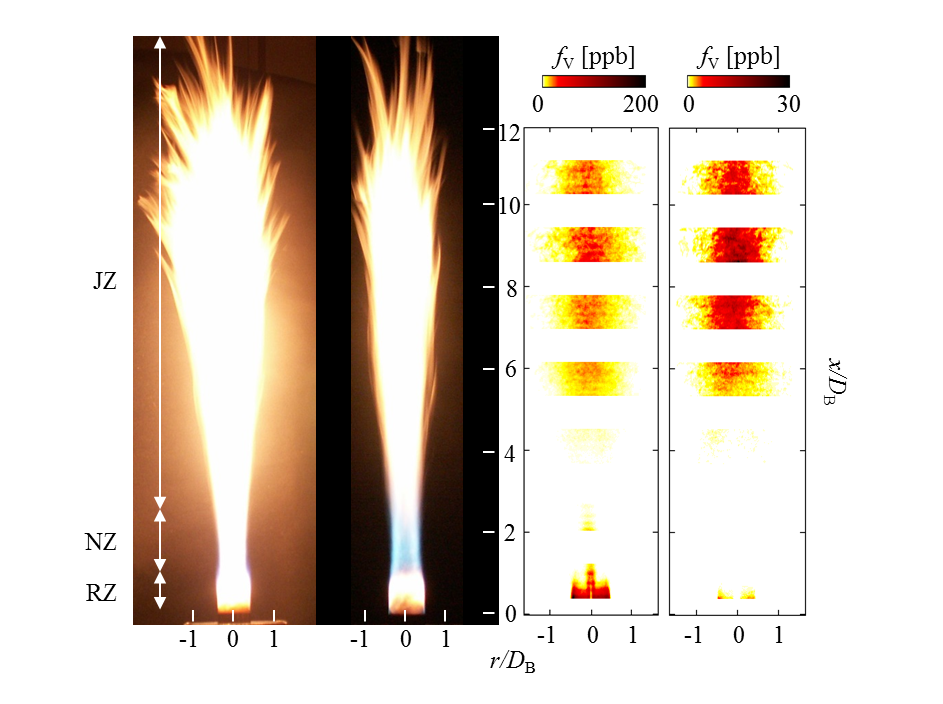
\includegraphics[trim=14mm 5.0mm 14mm 5mm, clip=true, width=0.5\textwidth]{hy_overall_new.png}
  \normalsize
  \vspace{-0.1in}
  \caption{Photographs of the neat ethylene (left) and ethylene/hydrogen (right) bluff body flame and the corresponding collages of the time-averaged LII images of the soot volume fraction distribution.  Three distinct regions are identified as follows: RZ (recirculation zone), NZ (neck zone), and JZ (jet-like zone).}
  \label{fig:H2_overall}
\end{figure}

Although the two flames share similar flow and soot formation patterns, the ethylene/hydrogen flame is significantly less sooting than the neat ethylene flame.  As demonstrated in Fig.~\ref{fig:ifv}, the axial profiles of the radially integrated soot volume fraction (ppm$\cdot$mm$^2$) are compared for the two flames.  Two distinct maxima are observed for both flames and correspond to the upstream recirculation zone and downstream jet-like zone.  Furthermore, the reduction in the integrated soot volume fraction is more pronounced in the recirculation zone than in the downstream jet-like region.  Specifically, according to both Figs.~\ref{fig:H2_overall} and~\ref{fig:ifv}, the soot reduction in the recirculation zone is more than an order of magnitude, while, in the jet-like zone, the reduction is about a factor of four to six.  The difference in the soot reduction with hydrogen addition indicates different \textcolor{Rv1}{dominant} soot reduction mechanisms and different roles that hydrogen addition plays in these two regions.  

\begin{figure}[t]
  \centering
  \scriptsize
  \vspace{-0.10in}
  \resizebox{0.5\textwidth}{!}{% GNUPLOT: LaTeX picture with Postscript
\begingroup
  \makeatletter
  \providecommand\color[2][]{%
    \GenericError{(gnuplot) \space\space\space\@spaces}{%
      Package color not loaded in conjunction with
      terminal option `colourtext'%
    }{See the gnuplot documentation for explanation.%
    }{Either use 'blacktext' in gnuplot or load the package
      color.sty in LaTeX.}%
    \renewcommand\color[2][]{}%
  }%
  \providecommand\includegraphics[2][]{%
    \GenericError{(gnuplot) \space\space\space\@spaces}{%
      Package graphicx or graphics not loaded%
    }{See the gnuplot documentation for explanation.%
    }{The gnuplot epslatex terminal needs graphicx.sty or graphics.sty.}%
    \renewcommand\includegraphics[2][]{}%
  }%
  \providecommand\rotatebox[2]{#2}%
  \@ifundefined{ifGPcolor}{%
    \newif\ifGPcolor
    \GPcolortrue
  }{}%
  \@ifundefined{ifGPblacktext}{%
    \newif\ifGPblacktext
    \GPblacktexttrue
  }{}%
  % define a \g@addto@macro without @ in the name:
  \let\gplgaddtomacro\g@addto@macro
  % define empty templates for all commands taking text:
  \gdef\gplbacktext{}%
  \gdef\gplfronttext{}%
  \makeatother
  \ifGPblacktext
    % no textcolor at all
    \def\colorrgb#1{}%
    \def\colorgray#1{}%
  \else
    % gray or color?
    \ifGPcolor
      \def\colorrgb#1{\color[rgb]{#1}}%
      \def\colorgray#1{\color[gray]{#1}}%
      \expandafter\def\csname LTw\endcsname{\color{white}}%
      \expandafter\def\csname LTb\endcsname{\color{black}}%
      \expandafter\def\csname LTa\endcsname{\color{black}}%
      \expandafter\def\csname LT0\endcsname{\color[rgb]{1,0,0}}%
      \expandafter\def\csname LT1\endcsname{\color[rgb]{0,1,0}}%
      \expandafter\def\csname LT2\endcsname{\color[rgb]{0,0,1}}%
      \expandafter\def\csname LT3\endcsname{\color[rgb]{1,0,1}}%
      \expandafter\def\csname LT4\endcsname{\color[rgb]{0,1,1}}%
      \expandafter\def\csname LT5\endcsname{\color[rgb]{1,1,0}}%
      \expandafter\def\csname LT6\endcsname{\color[rgb]{0,0,0}}%
      \expandafter\def\csname LT7\endcsname{\color[rgb]{1,0.3,0}}%
      \expandafter\def\csname LT8\endcsname{\color[rgb]{0.5,0.5,0.5}}%
    \else
      % gray
      \def\colorrgb#1{\color{black}}%
      \def\colorgray#1{\color[gray]{#1}}%
      \expandafter\def\csname LTw\endcsname{\color{white}}%
      \expandafter\def\csname LTb\endcsname{\color{black}}%
      \expandafter\def\csname LTa\endcsname{\color{black}}%
      \expandafter\def\csname LT0\endcsname{\color{black}}%
      \expandafter\def\csname LT1\endcsname{\color{black}}%
      \expandafter\def\csname LT2\endcsname{\color{black}}%
      \expandafter\def\csname LT3\endcsname{\color{black}}%
      \expandafter\def\csname LT4\endcsname{\color{black}}%
      \expandafter\def\csname LT5\endcsname{\color{black}}%
      \expandafter\def\csname LT6\endcsname{\color{black}}%
      \expandafter\def\csname LT7\endcsname{\color{black}}%
      \expandafter\def\csname LT8\endcsname{\color{black}}%
    \fi
  \fi
  \setlength{\unitlength}{0.0500bp}%
  \begin{picture}(4320.00,3024.00)%
    \gplgaddtomacro\gplbacktext{%
      \csname LTb\endcsname%
      \put(946,704){\makebox(0,0)[r]{\strut{} 0}}%
      \put(946,1218){\makebox(0,0)[r]{\strut{} 200}}%
      \put(946,1732){\makebox(0,0)[r]{\strut{} 400}}%
      \put(946,2245){\makebox(0,0)[r]{\strut{} 600}}%
      \put(946,2759){\makebox(0,0)[r]{\strut{} 800}}%
      \put(1078,484){\makebox(0,0){\strut{} 0}}%
      \put(1552,484){\makebox(0,0){\strut{} 2}}%
      \put(2026,484){\makebox(0,0){\strut{} 4}}%
      \put(2501,484){\makebox(0,0){\strut{} 6}}%
      \put(2975,484){\makebox(0,0){\strut{} 8}}%
      \put(3449,484){\makebox(0,0){\strut{} 10}}%
      \put(3923,484){\makebox(0,0){\strut{} 12}}%
      \put(176,1731){\rotatebox{-270}{\makebox(0,0){\strut{}\vspace{-28pt}Radially Integrated $f_{\rm V}$ [ppm$\cdot$mm$^2$] Per Unit Height}}}%
      \put(2500,154){\makebox(0,0){\strut{}$x/D_{\rm B}$}}%
    }%
    \gplgaddtomacro\gplfronttext{%
      \csname LTb\endcsname%
      \put(2936,2586){\makebox(0,0)[r]{\strut{}Ethylene}}%
      \csname LTb\endcsname%
      \put(2936,2366){\makebox(0,0)[r]{\strut{}Ethylene/Hydrogen}}%
    }%
    \gplbacktext
    \put(0,0){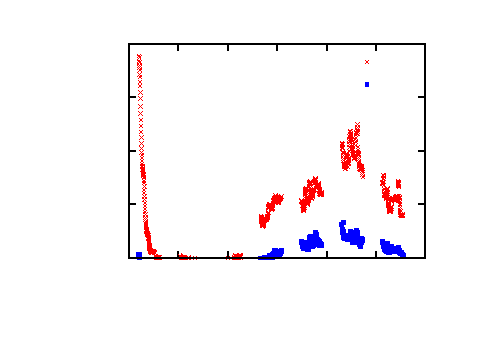
\includegraphics{ifv}}%
    \gplfronttext
  \end{picture}%
\endgroup
}
  \normalsize
  \vspace{-0.3in}
  \caption{Total soot volume per unit height obtained from the radial integration of the time-averaged soot volume fraction from the LII measurements at each height.  For clarity, only every second measurement point is shown.}
  \label{fig:ifv}
\end{figure}


\subsection{Effects of hydrogen addition}

Two effects of hydrogen addition are potentially relevant: chemical and hydrodynamic effects.  Chemically, due to the reduced C/H ratio, PAH formation will be inhibited in the hydrogen added flame, and, therefore, soot formation is inhibited.  \textcolor{Rv1}{This chemical effect is an intrinsic property of the fuel mixture, which is less dependent on the specific flow geometry compared to the hydrodynamic effect.  }Hydrodynamically, since the fuel jet velocity is increased, the fuel jet to air coflow momentum flux ratio is also increased\textcolor{Rv1}{ from 10.1 to 13.2}.  As Dally~\emph{et al.}~\cite{dally98b} demonstrated, the increase in the fuel jet momentum flux decreases the strength of the mixture in the outer vortex in the recirculation zone, further inhibiting soot formation.  The relative significance of these two effects in the two sooting regions of the flames are analyzed in this section.

To first quantify the chemical effect, steady flamelets at a moderate scalar dissipation rate ($\chi_{\rm st} = 1$ s$^{-1}$) were calculated, and the total PAH mass fraction is shown in Fig.~\ref{fig:flamelet}.  PAH forms at rich mixture fractions (the stoichiometric mixture fraction for both cases is about $0.06$, differing by less than $5$\%) and peaks at $Z = 0.2$.  The maximum $Y_{\rm PAH}$ decreases by a factor of two with hydrogen addition.  \textcolor{Rv1}{The scalar dissipation rate of 1 s$^{-1}$ was chosen because the representative value is of this order.  At higher scalar dissipation rates, such as 10 s$^{-1}$, PAH reduction with hydrogen addition is approximately the same, about a factor of 2.5.  At lower scalar dissipation rates, PAH shows substantial departure from the steady flamelet model~\cite{bisetti12}, so such scaling would not be expected to apply.  }In the soot model adopted in the LES, PAH-based soot formation and growth, which has been shown to dominate in turbulent jet flames~\cite{bisetti12,attili14,attili15,mueller12,mueller13}, scales as the square of the PAH mass fraction.  Therefore, this chemical effect is expected to result in a reduction of soot volume fraction by a factor of four in the jet-like region.  This reduction is consistent with the experimental measurements, \textcolor{Rv1}{suggesting that chemical effects are primarily responsible for soot suppression in the downstream jet-like region.}

\begin{figure}[t]
  \centering
  \scriptsize
  \resizebox{0.5\textwidth}{!}{% GNUPLOT: LaTeX picture with Postscript
\begingroup
  \makeatletter
  \providecommand\color[2][]{%
    \GenericError{(gnuplot) \space\space\space\@spaces}{%
      Package color not loaded in conjunction with
      terminal option `colourtext'%
    }{See the gnuplot documentation for explanation.%
    }{Either use 'blacktext' in gnuplot or load the package
      color.sty in LaTeX.}%
    \renewcommand\color[2][]{}%
  }%
  \providecommand\includegraphics[2][]{%
    \GenericError{(gnuplot) \space\space\space\@spaces}{%
      Package graphicx or graphics not loaded%
    }{See the gnuplot documentation for explanation.%
    }{The gnuplot epslatex terminal needs graphicx.sty or graphics.sty.}%
    \renewcommand\includegraphics[2][]{}%
  }%
  \providecommand\rotatebox[2]{#2}%
  \@ifundefined{ifGPcolor}{%
    \newif\ifGPcolor
    \GPcolortrue
  }{}%
  \@ifundefined{ifGPblacktext}{%
    \newif\ifGPblacktext
    \GPblacktexttrue
  }{}%
  % define a \g@addto@macro without @ in the name:
  \let\gplgaddtomacro\g@addto@macro
  % define empty templates for all commands taking text:
  \gdef\gplbacktext{}%
  \gdef\gplfronttext{}%
  \makeatother
  \ifGPblacktext
    % no textcolor at all
    \def\colorrgb#1{}%
    \def\colorgray#1{}%
  \else
    % gray or color?
    \ifGPcolor
      \def\colorrgb#1{\color[rgb]{#1}}%
      \def\colorgray#1{\color[gray]{#1}}%
      \expandafter\def\csname LTw\endcsname{\color{white}}%
      \expandafter\def\csname LTb\endcsname{\color{black}}%
      \expandafter\def\csname LTa\endcsname{\color{black}}%
      \expandafter\def\csname LT0\endcsname{\color[rgb]{1,0,0}}%
      \expandafter\def\csname LT1\endcsname{\color[rgb]{0,1,0}}%
      \expandafter\def\csname LT2\endcsname{\color[rgb]{0,0,1}}%
      \expandafter\def\csname LT3\endcsname{\color[rgb]{1,0,1}}%
      \expandafter\def\csname LT4\endcsname{\color[rgb]{0,1,1}}%
      \expandafter\def\csname LT5\endcsname{\color[rgb]{1,1,0}}%
      \expandafter\def\csname LT6\endcsname{\color[rgb]{0,0,0}}%
      \expandafter\def\csname LT7\endcsname{\color[rgb]{1,0.3,0}}%
      \expandafter\def\csname LT8\endcsname{\color[rgb]{0.5,0.5,0.5}}%
    \else
      % gray
      \def\colorrgb#1{\color{black}}%
      \def\colorgray#1{\color[gray]{#1}}%
      \expandafter\def\csname LTw\endcsname{\color{white}}%
      \expandafter\def\csname LTb\endcsname{\color{black}}%
      \expandafter\def\csname LTa\endcsname{\color{black}}%
      \expandafter\def\csname LT0\endcsname{\color{black}}%
      \expandafter\def\csname LT1\endcsname{\color{black}}%
      \expandafter\def\csname LT2\endcsname{\color{black}}%
      \expandafter\def\csname LT3\endcsname{\color{black}}%
      \expandafter\def\csname LT4\endcsname{\color{black}}%
      \expandafter\def\csname LT5\endcsname{\color{black}}%
      \expandafter\def\csname LT6\endcsname{\color{black}}%
      \expandafter\def\csname LT7\endcsname{\color{black}}%
      \expandafter\def\csname LT8\endcsname{\color{black}}%
    \fi
  \fi
  \setlength{\unitlength}{0.0500bp}%
  \begin{picture}(4320.00,3024.00)%
    \gplgaddtomacro\gplbacktext{%
      \csname LTb\endcsname%
      \put(946,704){\makebox(0,0)[r]{\strut{} 0}}%
      \put(946,1115){\makebox(0,0)[r]{\strut{} 0.2}}%
      \put(946,1526){\makebox(0,0)[r]{\strut{} 0.4}}%
      \put(946,1937){\makebox(0,0)[r]{\strut{} 0.6}}%
      \put(946,2348){\makebox(0,0)[r]{\strut{} 0.8}}%
      \put(946,2759){\makebox(0,0)[r]{\strut{} 1}}%
      \put(1078,484){\makebox(0,0){\strut{} 0}}%
      \put(1647,484){\makebox(0,0){\strut{} 0.2}}%
      \put(2216,484){\makebox(0,0){\strut{} 0.4}}%
      \put(2785,484){\makebox(0,0){\strut{} 0.6}}%
      \put(3354,484){\makebox(0,0){\strut{} 0.8}}%
      \put(3923,484){\makebox(0,0){\strut{} 1}}%
      \put(176,1731){\rotatebox{-270}{\makebox(0,0){\strut{}\vspace{-28pt}$Y_{\rm PAH} \times 10^4 $}}}%
      \put(2500,154){\makebox(0,0){\strut{}$Z$}}%
    }%
    \gplgaddtomacro\gplfronttext{%
      \csname LTb\endcsname%
      \put(3359,2586){\makebox(0,0)[r]{\strut{}Ethylene}}%
      \csname LTb\endcsname%
      \put(3359,2366){\makebox(0,0)[r]{\strut{}Ethylene/Hydrogen}}%
    }%
    \gplbacktext
    \put(0,0){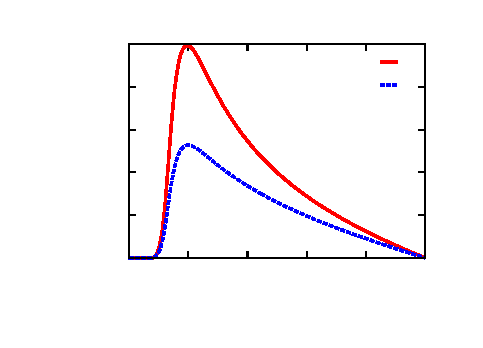
\includegraphics{ch-bluff/flamelet}}%
    \gplfronttext
  \end{picture}%
\endgroup
}
  \normalsize
  \vspace{-0.3in}
  \caption{PAH mass fraction profiles calculated with steady flamelets at $\chi = 1$ s$^{-1}$.}
  \label{fig:flamelet}
\end{figure}


Conversely, noting that the chemical effect predicted by the steady flamelet solution is less than the total soot reduction in the recirculation zone, soot evolution in this region is further analyzed with LES.  Radial profiles of the time-averaged soot volume fraction are shown in Fig.~\ref{fig:fv_radial} for both cases and at two axial locations in the recirculation zone.  Qualitatively, two distinct sooting peaks are found in the radial profiles.  Mueller~\emph{et al.}~\cite{mueller13} found in the ethylene bluff body flame that the inner and outer peak corresponds to the PAH-based growth and acetylene-based surface growth pathway, respectively.  Quantitatively, the \textcolor{Rv1}{calculated} soot volume fraction of the ethylene case is slightly underpredicted but within experimental uncertainty~\cite{mueller13}.  For the hydrogen added case, the \textcolor{Rv1}{calculated }soot volume fraction appears to be overpredicted.  However, the mean soot volume fraction from the LES is only slightly higher than the experimental detection limit of 3 ppb.  Therefore, the LII measurements may \textcolor{Rv1}{underquantify} the soot volume fraction by as much as 3 ppb, which easily accounts for the discrepancy between the measurements and LES.  \textcolor{Rv1}{An additional explanation could be that the recirculation zone is slightly too rich in the LES compared to the experiment, for which experimental diagnostics are only recently available~\cite{buxton13} and have not been applied to this flame.}

%\begin{figure}[t]
%  \centering
%  \scriptsize
%  \vspace{-0.10in}
%  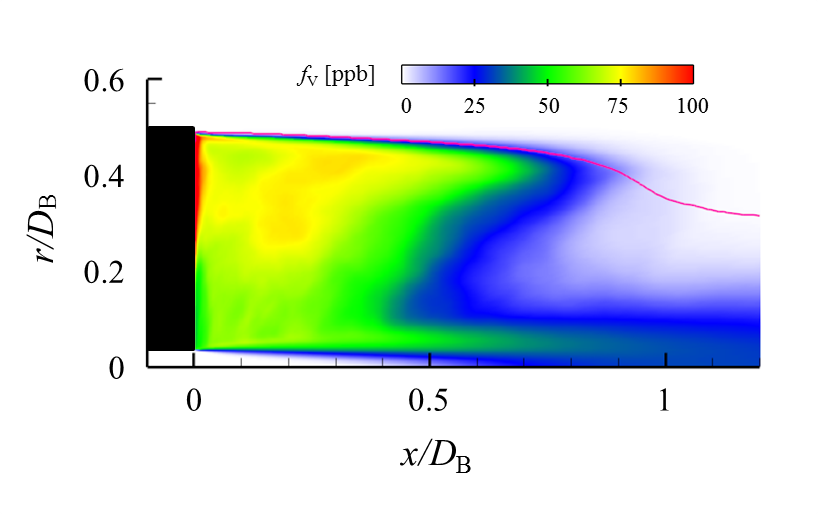
\includegraphics[trim=0mm 1.0mm 0mm 0.5mm, clip=true, width=0.5\textwidth]{ethy_fv.png}
%  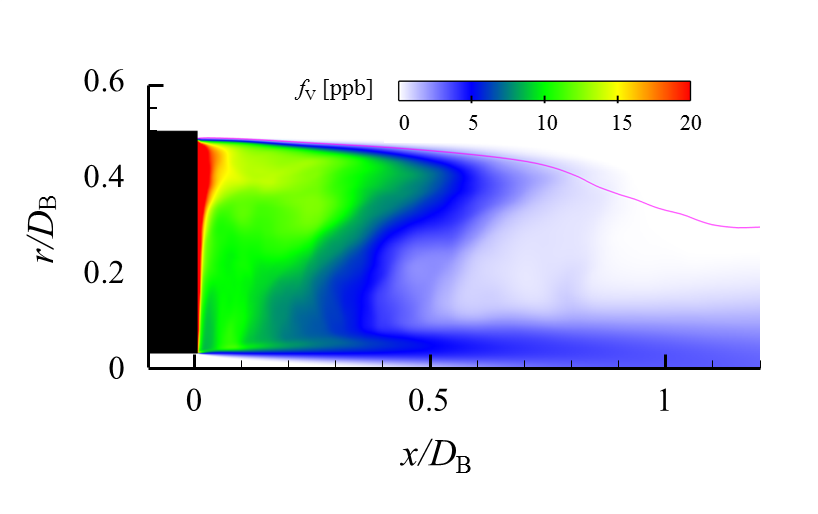
\includegraphics[trim=0mm 1.0mm 0mm 0.5mm, clip=true, width=0.5\textwidth]{hy_fv.png}
%  \normalsize
%  \vspace{-0.2in}
%  \caption{Time-averaged soot volume fraction [ppb] in the recirculation zone of the neat ethylene (top) and ethylene/hydrogen (bottom) flames.  The magenta line correspond to the stoichiometric mixture fraction contour.}
%  \label{fig:fv_RZ}
%\end{figure}

\begin{figure}[t]
  \centering
  \scriptsize
  \resizebox{0.49\textwidth}{!}{% GNUPLOT: LaTeX picture with Postscript
\begingroup
  \makeatletter
  \providecommand\color[2][]{%
    \GenericError{(gnuplot) \space\space\space\@spaces}{%
      Package color not loaded in conjunction with
      terminal option `colourtext'%
    }{See the gnuplot documentation for explanation.%
    }{Either use 'blacktext' in gnuplot or load the package
      color.sty in LaTeX.}%
    \renewcommand\color[2][]{}%
  }%
  \providecommand\includegraphics[2][]{%
    \GenericError{(gnuplot) \space\space\space\@spaces}{%
      Package graphicx or graphics not loaded%
    }{See the gnuplot documentation for explanation.%
    }{The gnuplot epslatex terminal needs graphicx.sty or graphics.sty.}%
    \renewcommand\includegraphics[2][]{}%
  }%
  \providecommand\rotatebox[2]{#2}%
  \@ifundefined{ifGPcolor}{%
    \newif\ifGPcolor
    \GPcolortrue
  }{}%
  \@ifundefined{ifGPblacktext}{%
    \newif\ifGPblacktext
    \GPblacktexttrue
  }{}%
  % define a \g@addto@macro without @ in the name:
  \let\gplgaddtomacro\g@addto@macro
  % define empty templates for all commands taking text:
  \gdef\gplbacktext{}%
  \gdef\gplfronttext{}%
  \makeatother
  \ifGPblacktext
    % no textcolor at all
    \def\colorrgb#1{}%
    \def\colorgray#1{}%
  \else
    % gray or color?
    \ifGPcolor
      \def\colorrgb#1{\color[rgb]{#1}}%
      \def\colorgray#1{\color[gray]{#1}}%
      \expandafter\def\csname LTw\endcsname{\color{white}}%
      \expandafter\def\csname LTb\endcsname{\color{black}}%
      \expandafter\def\csname LTa\endcsname{\color{black}}%
      \expandafter\def\csname LT0\endcsname{\color[rgb]{1,0,0}}%
      \expandafter\def\csname LT1\endcsname{\color[rgb]{0,1,0}}%
      \expandafter\def\csname LT2\endcsname{\color[rgb]{0,0,1}}%
      \expandafter\def\csname LT3\endcsname{\color[rgb]{1,0,1}}%
      \expandafter\def\csname LT4\endcsname{\color[rgb]{0,1,1}}%
      \expandafter\def\csname LT5\endcsname{\color[rgb]{1,1,0}}%
      \expandafter\def\csname LT6\endcsname{\color[rgb]{0,0,0}}%
      \expandafter\def\csname LT7\endcsname{\color[rgb]{1,0.3,0}}%
      \expandafter\def\csname LT8\endcsname{\color[rgb]{0.5,0.5,0.5}}%
    \else
      % gray
      \def\colorrgb#1{\color{black}}%
      \def\colorgray#1{\color[gray]{#1}}%
      \expandafter\def\csname LTw\endcsname{\color{white}}%
      \expandafter\def\csname LTb\endcsname{\color{black}}%
      \expandafter\def\csname LTa\endcsname{\color{black}}%
      \expandafter\def\csname LT0\endcsname{\color{black}}%
      \expandafter\def\csname LT1\endcsname{\color{black}}%
      \expandafter\def\csname LT2\endcsname{\color{black}}%
      \expandafter\def\csname LT3\endcsname{\color{black}}%
      \expandafter\def\csname LT4\endcsname{\color{black}}%
      \expandafter\def\csname LT5\endcsname{\color{black}}%
      \expandafter\def\csname LT6\endcsname{\color{black}}%
      \expandafter\def\csname LT7\endcsname{\color{black}}%
      \expandafter\def\csname LT8\endcsname{\color{black}}%
    \fi
  \fi
  \setlength{\unitlength}{0.0500bp}%
  \begin{picture}(4320.00,3024.00)%
    \gplgaddtomacro\gplbacktext{%
      \csname LTb\endcsname%
      \put(946,704){\makebox(0,0)[r]{\strut{} 0}}%
      \put(946,1218){\makebox(0,0)[r]{\strut{} 50}}%
      \put(946,1732){\makebox(0,0)[r]{\strut{} 100}}%
      \put(946,2245){\makebox(0,0)[r]{\strut{} 150}}%
      \put(946,2759){\makebox(0,0)[r]{\strut{} 200}}%
      \put(1078,484){\makebox(0,0){\strut{} 0}}%
      \put(1647,484){\makebox(0,0){\strut{} 0.1}}%
      \put(2216,484){\makebox(0,0){\strut{} 0.2}}%
      \put(2785,484){\makebox(0,0){\strut{} 0.3}}%
      \put(3354,484){\makebox(0,0){\strut{} 0.4}}%
      \put(3923,484){\makebox(0,0){\strut{} 0.5}}%
      \put(176,1731){\rotatebox{-270}{\makebox(0,0){\strut{}\vspace{-28pt}$\langle f_V \rangle$ [ppb]}}}%
      \put(2500,154){\makebox(0,0){\strut{}$r/D_{\rm B}$}}%
      \put(1249,2605){\makebox(0,0)[l]{\strut{}$x/D_{\rm B} = 0.432$}}%
      \put(2842,1012){\makebox(0,0)[l]{\strut{}$\times 10$}}%
    }%
    \gplgaddtomacro\gplfronttext{%
    }%
    \gplbacktext
    \put(0,0){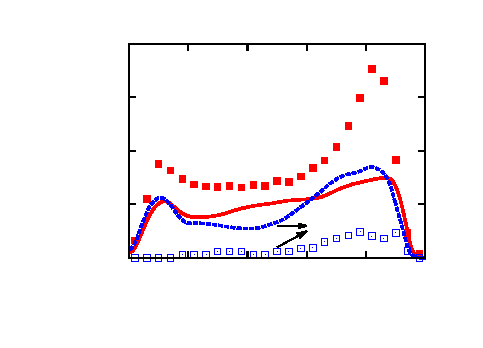
\includegraphics{ch-bluff/fv_06}}%
    \gplfronttext
  \end{picture}%
\endgroup
}
  \resizebox{0.49\textwidth}{!}{% GNUPLOT: LaTeX picture with Postscript
\begingroup
  \makeatletter
  \providecommand\color[2][]{%
    \GenericError{(gnuplot) \space\space\space\@spaces}{%
      Package color not loaded in conjunction with
      terminal option `colourtext'%
    }{See the gnuplot documentation for explanation.%
    }{Either use 'blacktext' in gnuplot or load the package
      color.sty in LaTeX.}%
    \renewcommand\color[2][]{}%
  }%
  \providecommand\includegraphics[2][]{%
    \GenericError{(gnuplot) \space\space\space\@spaces}{%
      Package graphicx or graphics not loaded%
    }{See the gnuplot documentation for explanation.%
    }{The gnuplot epslatex terminal needs graphicx.sty or graphics.sty.}%
    \renewcommand\includegraphics[2][]{}%
  }%
  \providecommand\rotatebox[2]{#2}%
  \@ifundefined{ifGPcolor}{%
    \newif\ifGPcolor
    \GPcolortrue
  }{}%
  \@ifundefined{ifGPblacktext}{%
    \newif\ifGPblacktext
    \GPblacktexttrue
  }{}%
  % define a \g@addto@macro without @ in the name:
  \let\gplgaddtomacro\g@addto@macro
  % define empty templates for all commands taking text:
  \gdef\gplbacktext{}%
  \gdef\gplfronttext{}%
  \makeatother
  \ifGPblacktext
    % no textcolor at all
    \def\colorrgb#1{}%
    \def\colorgray#1{}%
  \else
    % gray or color?
    \ifGPcolor
      \def\colorrgb#1{\color[rgb]{#1}}%
      \def\colorgray#1{\color[gray]{#1}}%
      \expandafter\def\csname LTw\endcsname{\color{white}}%
      \expandafter\def\csname LTb\endcsname{\color{black}}%
      \expandafter\def\csname LTa\endcsname{\color{black}}%
      \expandafter\def\csname LT0\endcsname{\color[rgb]{1,0,0}}%
      \expandafter\def\csname LT1\endcsname{\color[rgb]{0,1,0}}%
      \expandafter\def\csname LT2\endcsname{\color[rgb]{0,0,1}}%
      \expandafter\def\csname LT3\endcsname{\color[rgb]{1,0,1}}%
      \expandafter\def\csname LT4\endcsname{\color[rgb]{0,1,1}}%
      \expandafter\def\csname LT5\endcsname{\color[rgb]{1,1,0}}%
      \expandafter\def\csname LT6\endcsname{\color[rgb]{0,0,0}}%
      \expandafter\def\csname LT7\endcsname{\color[rgb]{1,0.3,0}}%
      \expandafter\def\csname LT8\endcsname{\color[rgb]{0.5,0.5,0.5}}%
    \else
      % gray
      \def\colorrgb#1{\color{black}}%
      \def\colorgray#1{\color[gray]{#1}}%
      \expandafter\def\csname LTw\endcsname{\color{white}}%
      \expandafter\def\csname LTb\endcsname{\color{black}}%
      \expandafter\def\csname LTa\endcsname{\color{black}}%
      \expandafter\def\csname LT0\endcsname{\color{black}}%
      \expandafter\def\csname LT1\endcsname{\color{black}}%
      \expandafter\def\csname LT2\endcsname{\color{black}}%
      \expandafter\def\csname LT3\endcsname{\color{black}}%
      \expandafter\def\csname LT4\endcsname{\color{black}}%
      \expandafter\def\csname LT5\endcsname{\color{black}}%
      \expandafter\def\csname LT6\endcsname{\color{black}}%
      \expandafter\def\csname LT7\endcsname{\color{black}}%
      \expandafter\def\csname LT8\endcsname{\color{black}}%
    \fi
  \fi
  \setlength{\unitlength}{0.0500bp}%
  \begin{picture}(4320.00,3024.00)%
    \gplgaddtomacro\gplbacktext{%
      \csname LTb\endcsname%
      \put(946,704){\makebox(0,0)[r]{\strut{} 0}}%
      \put(946,1218){\makebox(0,0)[r]{\strut{} 50}}%
      \put(946,1732){\makebox(0,0)[r]{\strut{} 100}}%
      \put(946,2245){\makebox(0,0)[r]{\strut{} 150}}%
      \put(946,2759){\makebox(0,0)[r]{\strut{} 200}}%
      \put(1078,484){\makebox(0,0){\strut{} 0}}%
      \put(1647,484){\makebox(0,0){\strut{} 0.1}}%
      \put(2216,484){\makebox(0,0){\strut{} 0.2}}%
      \put(2785,484){\makebox(0,0){\strut{} 0.3}}%
      \put(3354,484){\makebox(0,0){\strut{} 0.4}}%
      \put(3923,484){\makebox(0,0){\strut{} 0.5}}%
      \put(176,1731){\rotatebox{-270}{\makebox(0,0){\strut{}\vspace{-28pt}$\langle f_V \rangle$ [ppb]}}}%
      \put(2500,154){\makebox(0,0){\strut{}$r/D_{\rm B}$}}%
      \put(1249,2605){\makebox(0,0)[l]{\strut{}$x/D_{\rm B} = 0.576$}}%
      \put(3240,961){\makebox(0,0)[l]{\strut{}$\times 10$}}%
    }%
    \gplgaddtomacro\gplfronttext{%
      \csname LTb\endcsname%
      \put(2969,2322){\makebox(0,0)[r]{\strut{}Ethylene, LES}}%
      \csname LTb\endcsname%
      \put(2969,2168){\makebox(0,0)[r]{\strut{}Ethylene, Exp.}}%
      \csname LTb\endcsname%
      \put(2969,2014){\makebox(0,0)[r]{\strut{}Ethylene/Hydrogen, LES}}%
      \csname LTb\endcsname%
      \put(2969,1860){\makebox(0,0)[r]{\strut{}Ethylene/Hydrogen, Exp.}}%
    }%
    \gplbacktext
    \put(0,0){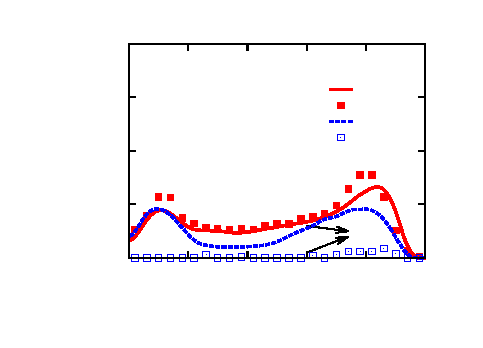
\includegraphics{ch-bluff/fv_08}}%
    \gplfronttext
  \end{picture}%
\endgroup
}
  \vspace{-0.3in}
  \normalsize
  \caption{Radial profiles of the time-averaged soot volume fraction.  Only every fourth experimental measurement point is shown for clarity.  The ethylene flame is reproduced from~\cite{mueller13}, and the ethylene/hydrogen flame is from this work.  Both experimental and computational results for the ethylene/hydrogen flame are scaled up by a factor of ten.}
  \label{fig:fv_radial}
\end{figure}

  
Hydrogen addition not only induces chemical effects through modification of the fuel stream C/H ratio but also hydrodynamically influences mixing, that is, the local mixture fraction, as well as residence time in the recirculation zone.  The residence time effect is first estimated by comparing the streamline patterns in the recirculation zone of the two flames, as shown in Fig.~\ref{fig:streamline}.  In both flames, the circulation vortex appears as single vortex near the outer shear layer between the air coflow and the recirculation zone due to sufficiently large jet/coflow momentum flux ratio~\cite{dally98a,dally98b}.  The location and structure of these two vortices are almost identical.  Estimating residence time~\cite{dally96} by dividing the length of the recirculation zone by the coflow velocity (identical between these flames), it is found that residence time in the recirculation zone is similar between these two flames.  Therefore, differences in residence time plays little role in dictating the difference in soot volume fraction in the recirculation zone in the two flames, and the difference beyond the chemical effects must be a result of different degrees of mixing in the recirculation zone.

\begin{figure}[t]
  \centering
  \scriptsize
  \vspace{-0.10in}
  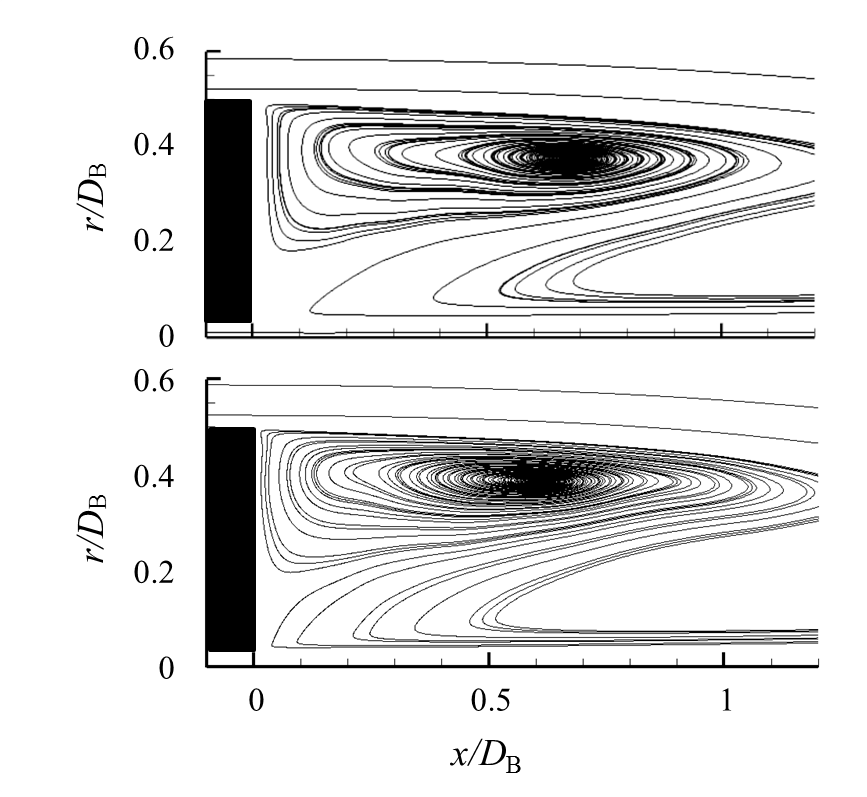
\includegraphics[trim=12.0mm 2.0mm 8mm 5mm, clip=true, width=0.35\textwidth]{streamline.png}
  \normalsize
  \vspace{-0.1in}
  \caption{Streamlines in the recirculation zone of the neat ethylene flame (top) and ethylene/hydrogen flame (bottom)~\textcolor{Rv1}{in the LES}.}
  \label{fig:streamline}
\end{figure}

\textcolor{Rv1}{The recirculating motion of the outer vortex transports rich mixture fraction from the fuel jet to the recirculation zone.  }As discussed above, the increase of the fuel/coflow momentum flux ratio~\textcolor{Rv1}{(about 30\%)} inhibits \textcolor{Rv1}{such transport}, resulting in a leaner recirculation zone than the neat ethylene case (recall that the stoichiometric mixture fraction is essentially the same for the two mixtures).  The mixture fraction radial profiles from LES as well as the characteristic time scales of the soot formation and oxidation processes from a lightly strained ($\chi_{\rm st} = 1$ s$^{-1}$) steady flamelet solution are shown in Fig.~\ref{fig:timescale}.  The characteristic time scales of the acetylene-based growth and oxidation processes remain the same, while that of the PAH-based growth slows down due to reduced PAH concentration as discussed previously.  Additionally, as expected, the mixture fraction profile near the bluff body surface is affected substantially by hydrogen addition.  As shown in Fig.~\ref{fig:timescale}, in the recirculation zone, the mean mixture fraction decreases by $25$\% with hydrogen addition.  Consequently, the mixture fraction shifts from where PAH-based growth is favored ($Z \sim 0.18$) to where oxidation becomes nearly as fast as acetylene-based surface growth ($Z \sim 0.11$), suppressing soot formation and growth.  Note that soot formation and oxidation are also sensitive to temperature, which is influenced by mixture fraction, gas-phase radiation, and soot radiation.  Due to the relatively low soot loading (ppb), soot radiation is negligible compared to gas-phase radiation, which depends on mixture fraction as well as residence time (same in both flames).  Therefore, the leaning in the recirculation zone due to hydrodynamic effects account for the further inhibited soot formation in addition to the chemical effect.

\begin{figure}[t]
  \centering
  \scriptsize
  \resizebox{0.49\textwidth}{!}{% GNUPLOT: LaTeX picture with Postscript
\begingroup
  \makeatletter
  \providecommand\color[2][]{%
    \GenericError{(gnuplot) \space\space\space\@spaces}{%
      Package color not loaded in conjunction with
      terminal option `colourtext'%
    }{See the gnuplot documentation for explanation.%
    }{Either use 'blacktext' in gnuplot or load the package
      color.sty in LaTeX.}%
    \renewcommand\color[2][]{}%
  }%
  \providecommand\includegraphics[2][]{%
    \GenericError{(gnuplot) \space\space\space\@spaces}{%
      Package graphicx or graphics not loaded%
    }{See the gnuplot documentation for explanation.%
    }{The gnuplot epslatex terminal needs graphicx.sty or graphics.sty.}%
    \renewcommand\includegraphics[2][]{}%
  }%
  \providecommand\rotatebox[2]{#2}%
  \@ifundefined{ifGPcolor}{%
    \newif\ifGPcolor
    \GPcolortrue
  }{}%
  \@ifundefined{ifGPblacktext}{%
    \newif\ifGPblacktext
    \GPblacktexttrue
  }{}%
  % define a \g@addto@macro without @ in the name:
  \let\gplgaddtomacro\g@addto@macro
  % define empty templates for all commands taking text:
  \gdef\gplbacktext{}%
  \gdef\gplfronttext{}%
  \makeatother
  \ifGPblacktext
    % no textcolor at all
    \def\colorrgb#1{}%
    \def\colorgray#1{}%
  \else
    % gray or color?
    \ifGPcolor
      \def\colorrgb#1{\color[rgb]{#1}}%
      \def\colorgray#1{\color[gray]{#1}}%
      \expandafter\def\csname LTw\endcsname{\color{white}}%
      \expandafter\def\csname LTb\endcsname{\color{black}}%
      \expandafter\def\csname LTa\endcsname{\color{black}}%
      \expandafter\def\csname LT0\endcsname{\color[rgb]{1,0,0}}%
      \expandafter\def\csname LT1\endcsname{\color[rgb]{0,1,0}}%
      \expandafter\def\csname LT2\endcsname{\color[rgb]{0,0,1}}%
      \expandafter\def\csname LT3\endcsname{\color[rgb]{1,0,1}}%
      \expandafter\def\csname LT4\endcsname{\color[rgb]{0,1,1}}%
      \expandafter\def\csname LT5\endcsname{\color[rgb]{1,1,0}}%
      \expandafter\def\csname LT6\endcsname{\color[rgb]{0,0,0}}%
      \expandafter\def\csname LT7\endcsname{\color[rgb]{1,0.3,0}}%
      \expandafter\def\csname LT8\endcsname{\color[rgb]{0.5,0.5,0.5}}%
    \else
      % gray
      \def\colorrgb#1{\color{black}}%
      \def\colorgray#1{\color[gray]{#1}}%
      \expandafter\def\csname LTw\endcsname{\color{white}}%
      \expandafter\def\csname LTb\endcsname{\color{black}}%
      \expandafter\def\csname LTa\endcsname{\color{black}}%
      \expandafter\def\csname LT0\endcsname{\color{black}}%
      \expandafter\def\csname LT1\endcsname{\color{black}}%
      \expandafter\def\csname LT2\endcsname{\color{black}}%
      \expandafter\def\csname LT3\endcsname{\color{black}}%
      \expandafter\def\csname LT4\endcsname{\color{black}}%
      \expandafter\def\csname LT5\endcsname{\color{black}}%
      \expandafter\def\csname LT6\endcsname{\color{black}}%
      \expandafter\def\csname LT7\endcsname{\color{black}}%
      \expandafter\def\csname LT8\endcsname{\color{black}}%
    \fi
  \fi
  \setlength{\unitlength}{0.0500bp}%
  \begin{picture}(4320.00,3024.00)%
    \gplgaddtomacro\gplbacktext{%
      \csname LTb\endcsname%
      \put(946,704){\makebox(0,0)[r]{\strut{} 0}}%
      \put(946,1115){\makebox(0,0)[r]{\strut{} 0.2}}%
      \put(946,1526){\makebox(0,0)[r]{\strut{} 0.4}}%
      \put(946,1937){\makebox(0,0)[r]{\strut{} 0.6}}%
      \put(946,2348){\makebox(0,0)[r]{\strut{} 0.8}}%
      \put(946,2759){\makebox(0,0)[r]{\strut{} 1}}%
      \put(1078,484){\makebox(0,0){\strut{} 0}}%
      \put(1647,484){\makebox(0,0){\strut{} 0.1}}%
      \put(2216,484){\makebox(0,0){\strut{} 0.2}}%
      \put(2785,484){\makebox(0,0){\strut{} 0.3}}%
      \put(3354,484){\makebox(0,0){\strut{} 0.4}}%
      \put(3923,484){\makebox(0,0){\strut{} 0.5}}%
      \put(176,1731){\rotatebox{-270}{\makebox(0,0){\strut{}\vspace{-28pt}$\langle Z \rangle$}}}%
      \put(2500,154){\makebox(0,0){\strut{}$r/D_{\rm B}$}}%
      \put(2785,1526){\makebox(0,0)[l]{\strut{}$x/D_{\rm B} = 0.072$}}%
    }%
    \gplgaddtomacro\gplfronttext{%
      \csname LTb\endcsname%
      \put(2936,2586){\makebox(0,0)[r]{\strut{}Ethylene}}%
      \csname LTb\endcsname%
      \put(2936,2366){\makebox(0,0)[r]{\strut{}Ethylene/Hydrogen}}%
    }%
    \gplbacktext
    \put(0,0){
\includegraphics{ch-bluff/Z_01}}%
    \gplfronttext
  \end{picture}%
\endgroup
}
  \resizebox{0.49\textwidth}{!}{% GNUPLOT: LaTeX picture with Postscript
\begingroup
  \makeatletter
  \providecommand\color[2][]{%
    \GenericError{(gnuplot) \space\space\space\@spaces}{%
      Package color not loaded in conjunction with
      terminal option `colourtext'%
    }{See the gnuplot documentation for explanation.%
    }{Either use 'blacktext' in gnuplot or load the package
      color.sty in LaTeX.}%
    \renewcommand\color[2][]{}%
  }%
  \providecommand\includegraphics[2][]{%
    \GenericError{(gnuplot) \space\space\space\@spaces}{%
      Package graphicx or graphics not loaded%
    }{See the gnuplot documentation for explanation.%
    }{The gnuplot epslatex terminal needs graphicx.sty or graphics.sty.}%
    \renewcommand\includegraphics[2][]{}%
  }%
  \providecommand\rotatebox[2]{#2}%
  \@ifundefined{ifGPcolor}{%
    \newif\ifGPcolor
    \GPcolortrue
  }{}%
  \@ifundefined{ifGPblacktext}{%
    \newif\ifGPblacktext
    \GPblacktexttrue
  }{}%
  % define a \g@addto@macro without @ in the name:
  \let\gplgaddtomacro\g@addto@macro
  % define empty templates for all commands taking text:
  \gdef\gplbacktext{}%
  \gdef\gplfronttext{}%
  \makeatother
  \ifGPblacktext
    % no textcolor at all
    \def\colorrgb#1{}%
    \def\colorgray#1{}%
  \else
    % gray or color?
    \ifGPcolor
      \def\colorrgb#1{\color[rgb]{#1}}%
      \def\colorgray#1{\color[gray]{#1}}%
      \expandafter\def\csname LTw\endcsname{\color{white}}%
      \expandafter\def\csname LTb\endcsname{\color{black}}%
      \expandafter\def\csname LTa\endcsname{\color{black}}%
      \expandafter\def\csname LT0\endcsname{\color[rgb]{1,0,0}}%
      \expandafter\def\csname LT1\endcsname{\color[rgb]{0,1,0}}%
      \expandafter\def\csname LT2\endcsname{\color[rgb]{0,0,1}}%
      \expandafter\def\csname LT3\endcsname{\color[rgb]{1,0,1}}%
      \expandafter\def\csname LT4\endcsname{\color[rgb]{0,1,1}}%
      \expandafter\def\csname LT5\endcsname{\color[rgb]{1,1,0}}%
      \expandafter\def\csname LT6\endcsname{\color[rgb]{0,0,0}}%
      \expandafter\def\csname LT7\endcsname{\color[rgb]{1,0.3,0}}%
      \expandafter\def\csname LT8\endcsname{\color[rgb]{0.5,0.5,0.5}}%
    \else
      % gray
      \def\colorrgb#1{\color{black}}%
      \def\colorgray#1{\color[gray]{#1}}%
      \expandafter\def\csname LTw\endcsname{\color{white}}%
      \expandafter\def\csname LTb\endcsname{\color{black}}%
      \expandafter\def\csname LTa\endcsname{\color{black}}%
      \expandafter\def\csname LT0\endcsname{\color{black}}%
      \expandafter\def\csname LT1\endcsname{\color{black}}%
      \expandafter\def\csname LT2\endcsname{\color{black}}%
      \expandafter\def\csname LT3\endcsname{\color{black}}%
      \expandafter\def\csname LT4\endcsname{\color{black}}%
      \expandafter\def\csname LT5\endcsname{\color{black}}%
      \expandafter\def\csname LT6\endcsname{\color{black}}%
      \expandafter\def\csname LT7\endcsname{\color{black}}%
      \expandafter\def\csname LT8\endcsname{\color{black}}%
    \fi
  \fi
  \setlength{\unitlength}{0.0500bp}%
  \begin{picture}(4320.00,3024.00)%
    \gplgaddtomacro\gplbacktext{%
      \csname LTb\endcsname%
      \put(814,704){\makebox(0,0)[r]{\strut{}$10^{1}$}}%
      \put(814,1218){\makebox(0,0)[r]{\strut{}$10^{2}$}}%
      \put(814,1732){\makebox(0,0)[r]{\strut{}$10^{3}$}}%
      \put(814,2245){\makebox(0,0)[r]{\strut{}$10^{4}$}}%
      \put(814,2759){\makebox(0,0)[r]{\strut{}$10^{5}$}}%
      \put(946,484){\makebox(0,0){\strut{} 0}}%
      \put(1541,484){\makebox(0,0){\strut{} 0.1}}%
      \put(2137,484){\makebox(0,0){\strut{} 0.2}}%
      \put(2732,484){\makebox(0,0){\strut{} 0.3}}%
      \put(3328,484){\makebox(0,0){\strut{} 0.4}}%
      \put(3923,484){\makebox(0,0){\strut{} 0.5}}%
      \put(176,1731){\rotatebox{-270}{\makebox(0,0){\strut{}\vspace{-28pt}$1$ / $\tau$ [1/s]}}}%
      \put(2434,154){\makebox(0,0){\strut{}$Z$}}%
      \put(1846,2555){\makebox(0,0)[l]{\strut{}Ethylene: solid}}%
      \put(1846,2295){\makebox(0,0)[l]{\strut{}Ethylene/Hydrogen: dashed}}%
      \put(1184,2195){\makebox(0,0)[l]{\strut{}Ox.}}%
      \put(1720,1886){\makebox(0,0)[l]{\strut{}S.G.}}%
      \put(2732,1218){\makebox(0,0)[l]{\strut{}Nucl. + Cond.}}%
    }%
    \gplgaddtomacro\gplfronttext{%
    }%
    \gplbacktext
    \put(0,0){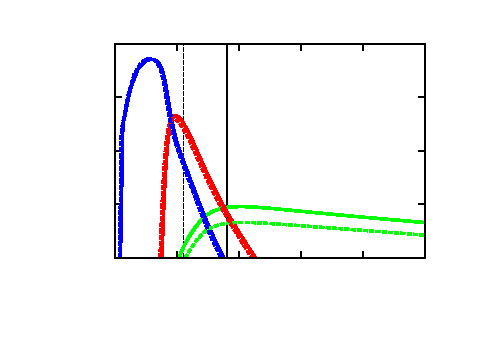
\includegraphics{ch-bluff/timescale}}%
    \gplfronttext
  \end{picture}%
\endgroup
}
  \vspace{-0.3in}
  \normalsize
  \caption{Left: radial profile of the time-averaged mixture fraction~\textcolor{Rv1}{in the LES at different heights.  Black horizontal} lines correspond to the stoichiometric mixture fractions of these two flames and almost overlap.  Right: characteristic inverse time scales of the soot processes from the steady flamelet calculations at $\chi_{\rm st} = 1$ s$^{-1}$.  Vertical lines correspond to the mixture fraction in the flat regions of the radial plot.}
  \label{fig:timescale}
\end{figure}

The PAH-based, acetylene-based, and oxidation source terms are shown in Fig.~\ref{fig:sourceterms} to elucidate the evolution of soot. Soot nucleation mainly occurs near the inner shear layer between the fuel jet and recirculation zone where mixture fraction is high.  Some of this soot is entrained by the recirculation zone and transported back upstream toward the bluff body then radially outward toward the outer shear layer by the recirculation vortex.  This trend is consistent with the neat ethylene case~\cite{mueller13}.  In the neat ethylene flame, acetylene-based surface growth becomes dominant in the outer shear layer close to the stoichiometric mixture fraction contour, and oxidation is almost negligible except close to the downstream neck zone.  However, due to the lean shift of the mean mixture fraction near the bluff body in the hydrogen added flame, oxidation becomes comparable to the acetylene-based growth.  Consequently, soot nucleation in the recirculation zone of the hydrogen added flame is first suppressed due to reduced PAH concentration, and soot surface growth competes with soot oxidation, resulting in a less sooting recirculation zone than the neat ethylene flame.

 \begin{figure}[t]
  \centering
  \scriptsize
  \vspace{-0.10in}
  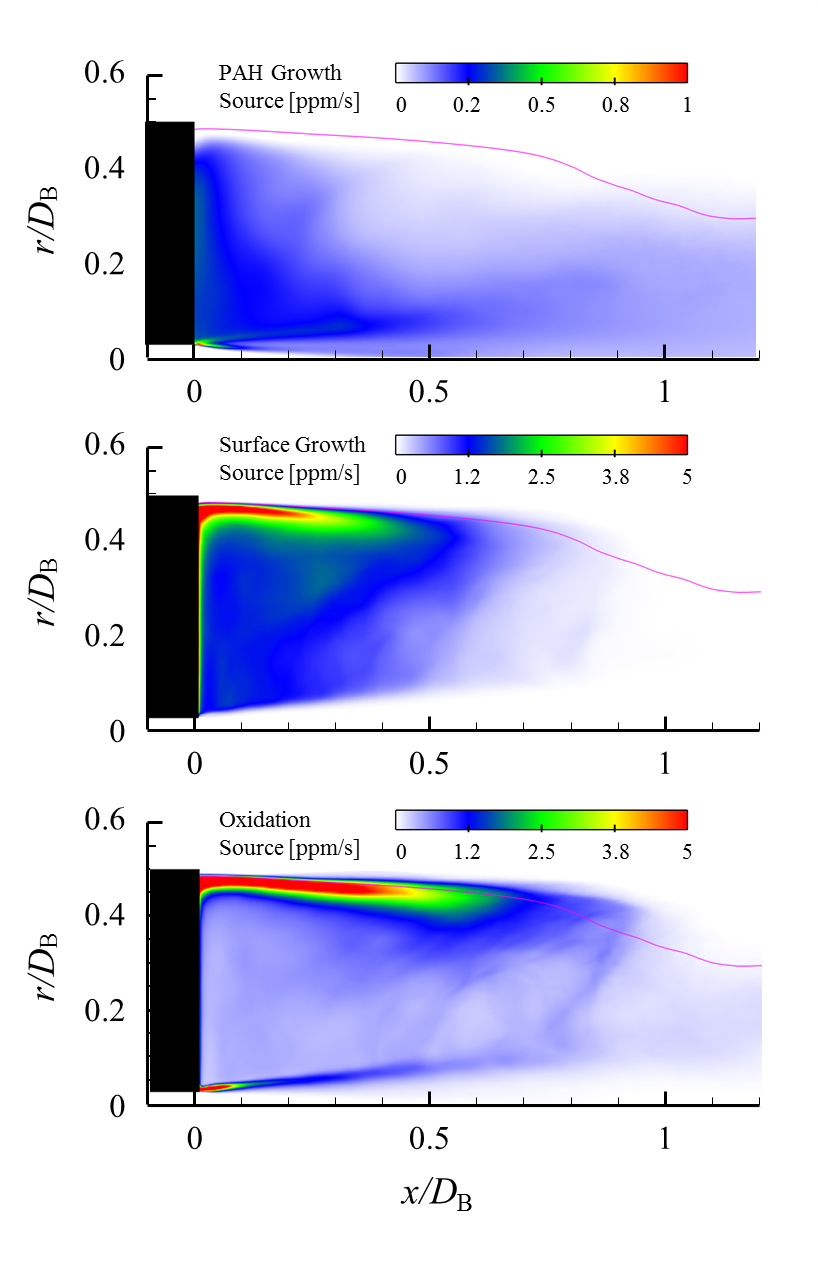
\includegraphics[trim=5mm 5.0mm 10mm 3.0mm, clip=true, width=0.4\textwidth]{sourceterm.png}
  \normalsize
  \vspace{-0.2in}
  \caption{Time-averaged soot volume fraction source term [ppm/s] in the recirculation zone of the ethylene/hydrogen flame~\textcolor{Rv1}{in the LES}.  The magenta lines correspond to the stoichiometric mixture fraction contours.}
  \label{fig:sourceterms}
\end{figure}

%====================================================================

\section{Conclusions}

A sooting turbulent bluff body stabilized ethylene/hydrogen flame was studied both experimentally and computationally and compared with a previously analyzed neat ethylene counterpart~\cite{mueller13}.  Laser-induced incandescence (LII) was utilized to measure the soot volume fraction in the flame.  An integrated Large Eddy Simulation (LES) model was adopted to elucidate the interactions between soot, turbulence, and chemistry.  The statistical soot model was based on the Hybrid Method of Moments (HMOM), considering detailed nucleation, condensation, particle collision, surface growth, oxidation, and fragmentation processes that influence soot evolution.  The combustion model for the gas-phase was based on the Radiation Flamelet/Progress Variable (RFPV) model with modifications to account for the removal of Polycyclic Aromatic Hydrocarbon (PAH) from the gas-phase.  A presumed PDF was utilized to model unresolved subfilter scale interactions.

Similar to the neat ethylene bluff body flame, three distinct flow regions were observed experimentally: a sooting recirculation zone, a non-sooting, high-strain neck region, and a sooting jet-like zone.  Although the ethylene/hydrogen case is significantly less sooting than the neat ethylene counterpart overall, soot reduction in the recirculation zone near the bluff body is more pronounced than in the downstream jet-like region.  Both chemical and hydrodynamic effects were identified as reasons for this decrease.

The chemical effect was first quantified from a steady flamelet calculation.  Due to the hydrogen addition, PAH mass fraction was found to decrease by a factor of two, indicating a factor of four decrease in the PAH-based growth rate that includes both nucleation and PAH condensation.  This is consistent with the soot reduction in the downstream jet-like region, where PAH-based growth is dominant.  Therefore, the chemical effect is dominant in this region.

The hydrodynamic effect was then analyzed, since both the experimental measurements and LES calculations demonstrated additional soot reduction in the recirculation zone, which could not be explained with the chemical effect alone.  The streamline patterns in the recirculation zone of the two flames are similar according to LES, and therefore, differences in residence time plays little role in the difference in soot volume fraction in the recirculation zone.  

Conversely, in the experiment, to attain the same \textcolor{Rv1}{heat release rate and similar }Reynolds number in the hydrogen added flame as the neat ethylene flame, the central jet velocity was increased.  This increase in the fuel to air coflow momentum flux ratio entrains less fuel into the recirculation zone near the bluff body surface, compared to the neat ethylene flame.  Due to the leaner mixture fraction in the recirculation zone, soot nucleation and surface growth is inhibited and soot oxidation is promoted.  This hydrodynamic effect together with the chemical effect accounts for the soot reduction in the recirculation zone.    

\section*{Acknowledgments}

The Australian authors gratefully acknowledge funding from the Australian Research Council (ARC) through the Discovery and the Linkage Infrastructure, Equipment, and Facilities (LIEF) grant programs.

%====================================================================

\section*{References}
\bibliographystyle{elsarticle-num-PCI}
\bibliography{bluff}

\renewcommand{\thefigure}{\arabic{figure}}
\renewcommand{\thetable}{\arabic{table}}

\clearpage
\listoffigures

\end{document}





  
